% GNUPLOT: LaTeX picture with Postscript
\begingroup
  \makeatletter
  \providecommand\color[2][]{%
    \GenericError{(gnuplot) \space\space\space\@spaces}{%
      Package color not loaded in conjunction with
      terminal option `colourtext'%
    }{See the gnuplot documentation for explanation.%
    }{Either use 'blacktext' in gnuplot or load the package
      color.sty in LaTeX.}%
    \renewcommand\color[2][]{}%
  }%
  \providecommand\includegraphics[2][]{%
    \GenericError{(gnuplot) \space\space\space\@spaces}{%
      Package graphicx or graphics not loaded%
    }{See the gnuplot documentation for explanation.%
    }{The gnuplot epslatex terminal needs graphicx.sty or graphics.sty.}%
    \renewcommand\includegraphics[2][]{}%
  }%
  \providecommand\rotatebox[2]{#2}%
  \@ifundefined{ifGPcolor}{%
    \newif\ifGPcolor
    \GPcolortrue
  }{}%
  \@ifundefined{ifGPblacktext}{%
    \newif\ifGPblacktext
    \GPblacktexttrue
  }{}%
  % define a \g@addto@macro without @ in the name:
  \let\gplgaddtomacro\g@addto@macro
  % define empty templates for all commands taking text:
  \gdef\gplbacktext{}%
  \gdef\gplfronttext{}%
  \makeatother
  \ifGPblacktext
    % no textcolor at all
    \def\colorrgb#1{}%
    \def\colorgray#1{}%
  \else
    % gray or color?
    \ifGPcolor
      \def\colorrgb#1{\color[rgb]{#1}}%
      \def\colorgray#1{\color[gray]{#1}}%
      \expandafter\def\csname LTw\endcsname{\color{white}}%
      \expandafter\def\csname LTb\endcsname{\color{black}}%
      \expandafter\def\csname LTa\endcsname{\color{black}}%
      \expandafter\def\csname LT0\endcsname{\color[rgb]{1,0,0}}%
      \expandafter\def\csname LT1\endcsname{\color[rgb]{0,1,0}}%
      \expandafter\def\csname LT2\endcsname{\color[rgb]{0,0,1}}%
      \expandafter\def\csname LT3\endcsname{\color[rgb]{1,0,1}}%
      \expandafter\def\csname LT4\endcsname{\color[rgb]{0,1,1}}%
      \expandafter\def\csname LT5\endcsname{\color[rgb]{1,1,0}}%
      \expandafter\def\csname LT6\endcsname{\color[rgb]{0,0,0}}%
      \expandafter\def\csname LT7\endcsname{\color[rgb]{1,0.3,0}}%
      \expandafter\def\csname LT8\endcsname{\color[rgb]{0.5,0.5,0.5}}%
    \else
      % gray
      \def\colorrgb#1{\color{black}}%
      \def\colorgray#1{\color[gray]{#1}}%
      \expandafter\def\csname LTw\endcsname{\color{white}}%
      \expandafter\def\csname LTb\endcsname{\color{black}}%
      \expandafter\def\csname LTa\endcsname{\color{black}}%
      \expandafter\def\csname LT0\endcsname{\color{black}}%
      \expandafter\def\csname LT1\endcsname{\color{black}}%
      \expandafter\def\csname LT2\endcsname{\color{black}}%
      \expandafter\def\csname LT3\endcsname{\color{black}}%
      \expandafter\def\csname LT4\endcsname{\color{black}}%
      \expandafter\def\csname LT5\endcsname{\color{black}}%
      \expandafter\def\csname LT6\endcsname{\color{black}}%
      \expandafter\def\csname LT7\endcsname{\color{black}}%
      \expandafter\def\csname LT8\endcsname{\color{black}}%
    \fi
  \fi
    \setlength{\unitlength}{0.0500bp}%
    \ifx\gptboxheight\undefined%
      \newlength{\gptboxheight}%
      \newlength{\gptboxwidth}%
      \newsavebox{\gptboxtext}%
    \fi%
    \setlength{\fboxrule}{0.5pt}%
    \setlength{\fboxsep}{1pt}%
\begin{picture}(7200.00,5040.00)%
    \gplgaddtomacro\gplbacktext{%
      \csname LTb\endcsname%
      \put(814,704){\makebox(0,0)[r]{\strut{}$0$}}%
      \put(814,1518){\makebox(0,0)[r]{\strut{}$0.2$}}%
      \put(814,2332){\makebox(0,0)[r]{\strut{}$0.4$}}%
      \put(814,3147){\makebox(0,0)[r]{\strut{}$0.6$}}%
      \put(814,3961){\makebox(0,0)[r]{\strut{}$0.8$}}%
      \put(814,4775){\makebox(0,0)[r]{\strut{}$1$}}%
      \put(1457,484){\makebox(0,0){\strut{}$760$}}%
      \put(2479,484){\makebox(0,0){\strut{}$780$}}%
      \put(3501,484){\makebox(0,0){\strut{}$800$}}%
      \put(4522,484){\makebox(0,0){\strut{}$820$}}%
      \put(5544,484){\makebox(0,0){\strut{}$840$}}%
      \put(6187,1111){\makebox(0,0)[l]{\strut{}$-4$}}%
      \put(6187,1925){\makebox(0,0)[l]{\strut{}$-2$}}%
      \put(6187,2740){\makebox(0,0)[l]{\strut{}$0$}}%
      \put(6187,3554){\makebox(0,0)[l]{\strut{}$2$}}%
      \put(6187,4368){\makebox(0,0)[l]{\strut{}$4$}}%
    }%
    \gplgaddtomacro\gplfronttext{%
      \csname LTb\endcsname%
      \put(176,2739){\rotatebox{-270}{\makebox(0,0){\strut{}Spektrale Intensität $S$}}}%
      \put(6692,2739){\rotatebox{-270}{\makebox(0,0){\strut{}Phase $\Phi$ [rad]}}}%
      \put(3500,154){\makebox(0,0){\strut{}Wellenllänge $\lambda$ [nm]}}%
      \csname LTb\endcsname%
      \put(5068,4602){\makebox(0,0)[r]{\strut{}\tiny$S:0.95\;\text{nm}$}}%
      \csname LTb\endcsname%
      \put(5068,4382){\makebox(0,0)[r]{\strut{}\tiny$S:1.45\;\text{nm}$}}%
      \csname LTb\endcsname%
      \put(5068,4162){\makebox(0,0)[r]{\strut{}\tiny$S:1.95\;\text{nm}$}}%
      \csname LTb\endcsname%
      \put(5068,3942){\makebox(0,0)[r]{\strut{}\tiny$S:2.45\;\text{nm}$}}%
      \csname LTb\endcsname%
      \put(5068,3722){\makebox(0,0)[r]{\strut{}\tiny$S:2.84\;\text{nm}$}}%
      \csname LTb\endcsname%
      \put(5068,3502){\makebox(0,0)[r]{\strut{}\tiny$S:2.84\;\text{nm (opt)}$}}%
      \csname LTb\endcsname%
      \put(5068,3282){\makebox(0,0)[r]{\strut{}\tiny$\Phi:0.95\;\text{nm}$}}%
      \csname LTb\endcsname%
      \put(5068,3062){\makebox(0,0)[r]{\strut{}\tiny$\Phi:1.45\;\text{nm}$}}%
      \csname LTb\endcsname%
      \put(5068,2842){\makebox(0,0)[r]{\strut{}\tiny$\Phi:1.95\;\text{nm}$}}%
      \csname LTb\endcsname%
      \put(5068,2622){\makebox(0,0)[r]{\strut{}\tiny$\Phi:2.45\;\text{nm}$}}%
      \csname LTb\endcsname%
      \put(5068,2402){\makebox(0,0)[r]{\strut{}\tiny$\Phi:2.84\;\text{nm}$}}%
      \csname LTb\endcsname%
      \put(5068,2182){\makebox(0,0)[r]{\strut{}\tiny$\Phi:2.84\;\text{nm (opt)}$}}%
      \csname LTb\endcsname%
      \put(5068,1962){\makebox(0,0)[r]{\strut{}fit}}%
    }%
    \gplbacktext
    \put(0,0){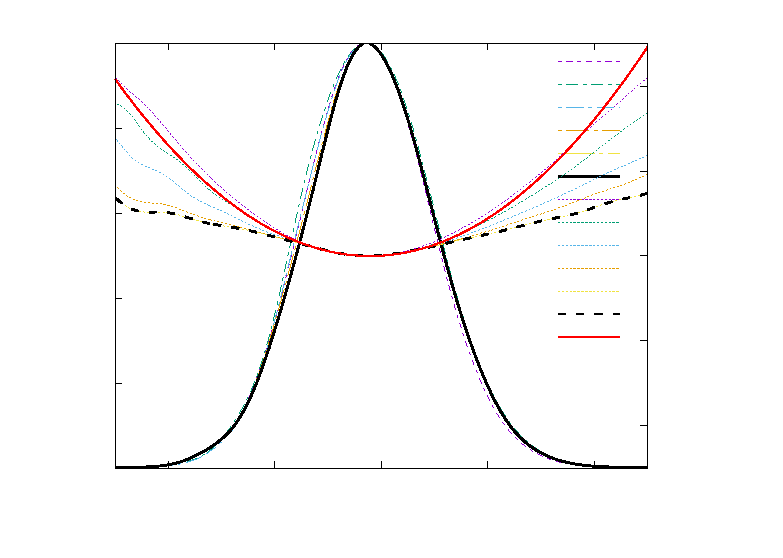
\includegraphics{spec2}}%
    \gplfronttext
  \end{picture}%
\endgroup
